\section{Introduction}
The case study used throughout this thesis is the need for indoor location and routing inside a hospital muiltifloor environment. In this chapter the needed actions to implement the usage of Cisco CMX inside an android application are discussed. Firstly, the mapping component, being MapWize, is discussed, followed by the part of indoor location tracking and an indoor location framework provided by IndoorLocation. Finally xxxxxxxxxxxxxx.
\section{MapWize}
MapWize is a company that allows developers of an indoor location application to translate architectural floor plans into a digital mapping. Not only do they convert the existing plans but also implement routing and specific points of interest. This eliminates the need for a specific developer team of the company or agency that implements this systems as this is part of the service MapWize provides.
MORE ON FEATURES
\section{MapWize Competitors}
\subsection{MazeMap}
MazeMap offers a digital platform to create and editor architectural maps. One of their biggest advantages is the fact that they can incorporate changes in their digital maps based on a .DWG or .DXF file, which is the used file format for \acrfull{cad} applications \cite{Coon2015}. Other than that it offers positioning and wayfinding by integrating the Cisco \acrlong{cmx} technology. Moreover, MazeMap provides an \acrshort{api} to integrate legacy software or other applications, such as Outlook Exchange, into the ecosystem of indoor location \cite{MazeMapb} \cite{MazeMapa}. An additional feature is the ability to add \acrfull{iot}-driven devices and sensors to enable asset tracking.
\subparagraph{Case study of Bergen University College}
One of the case studies performed by Cisco is the implementation of Cisco CMX inside the Bergen \acrshort{uc}. The goal of implementing Cisco CMX was to provide students with a \acrfull{byod} policy by creating an 802.11ac WLAN that was scalable to provide each student with Internet access. As stated in the case study, the following devices were used \cite{Magrane2016}:
\begin{itemize}
\item Cisco Aironet 3702e and 3702i \acrlong{ap}s;
\item Cisco 5760 WLAN controllers;
\item Cisco 3850 and 4500-X Series switches;
\item Cisco Catalyst 6500 Series switches;
\end{itemize}
To enable students to use the wayfinding feature, Cisco partnered with MazeMap to create the service and keep it up-to-date with changes in the campus. The major benefit, as mentioned in the case study, is the elimination of crowded hallways that in its turn resulted in a higher, overall happiness amongst students of this \acrlong{uc}.
\begin{figure}[h!]
\centering
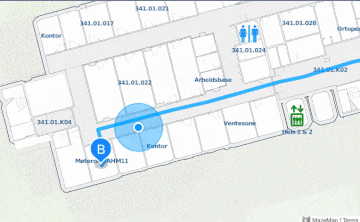
\includegraphics[scale=0.75]{mazemap_wayfinding}
\caption{Routing feature of MazeMap ~\cite{MazeMapa}}
\label{fig:ips_topologies}
\end{figure}
\begin{figure}[h!]
\centering
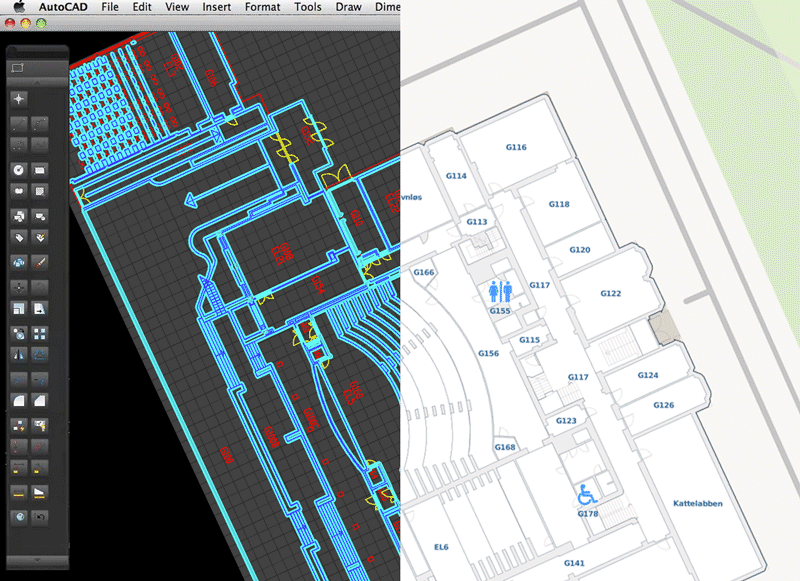
\includegraphics[scale=0.3]{mazemap_mapping}
\caption{Translating floor plans into an interactive map for MazeMap ~\cite{MazeMap}}
\label{fig:ips_topologies}
\end{figure}
\subsection{MapsIndoors}
Another company providing digital indoor mapping is MapsIndoors. This company focuses on providing an ecosystem of both routing and indoor maps by offering a \acrfull{cms} and a cloud environment that serves the indoor navigation platform. Other than a \acrshort{sdk} they implemented a data \acrshort{api} to allow statistics to be drawn from user data and allowing existing systems, such are booking, \acrfull{erp} and \acrfull{crm} systems, to use this data to analyse and visualize. On their website, there is no indication of price or the specific indoor location techniques used in the service. The unique feature of MapsIndoors, as stated on their website, is the seamless integration of outdoor navigation based on Google Maps and indoor navigation, which is resemblant to Google Maps \cite{MapsIndoors}.
\begin{figure}[h!]
\centering
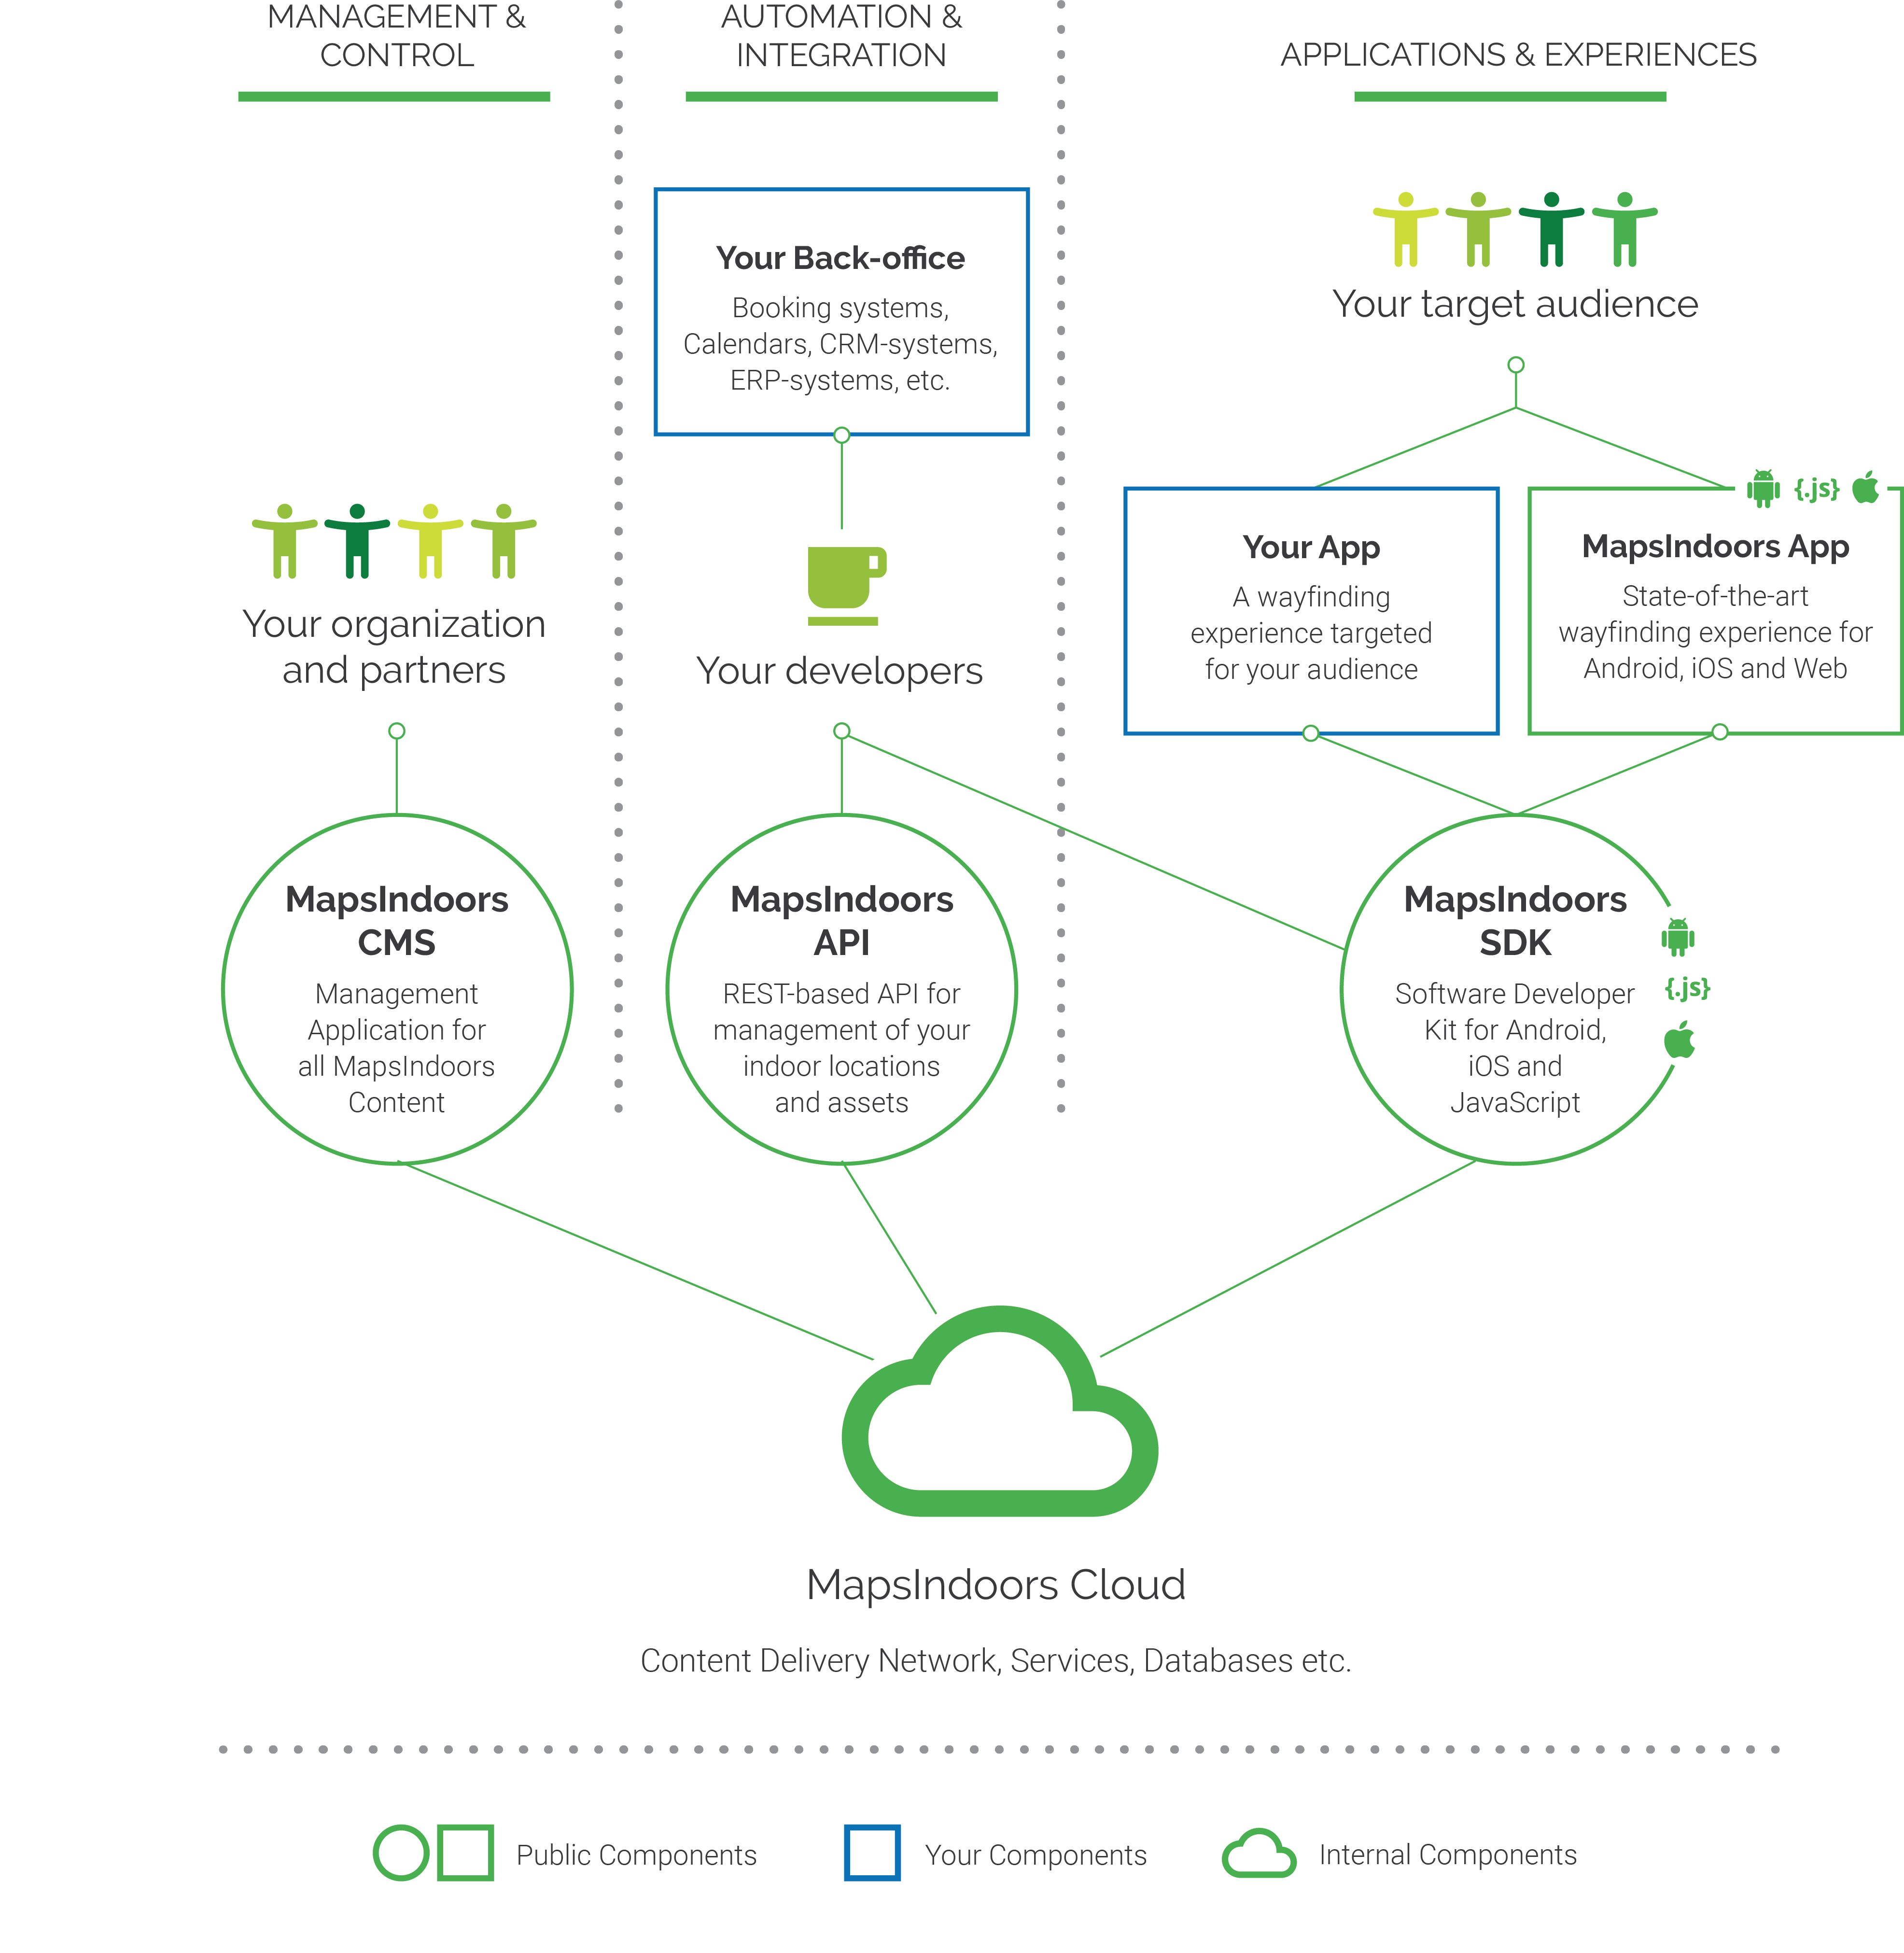
\includegraphics[scale=0.4]{mapsindoors_architecture}
\caption{Architecture of the MapsIndoors platform ~\cite{MapsIndoors}}
\label{fig:ips_topologies}
\end{figure}
\subsection{Google Indoor Maps}
Google Indoor Maps is a free service to create an interactive map of an environment. It is based on the Google Maps \acrshort{ui} with the corresponding universal icons and allows users to navigate inside a building. There is however no indication of which technology used to accurately display a user's position. As this is a Google product, developers can expect an easy-to-use \acrshort{api} with sufficient code examples and documentation as well as cross-platform integrations: web, Apple and Android applications. A downside to this service is that changes to a digital map are not easily applied, the different offices of Google responsible for applying changes need to be notified of the changes, which can presumably result in some waiting time.
Other than that disadvantage, this service offers a free alternative to other competitors \cite{Google}.
\begin{figure}[h!]
\centering
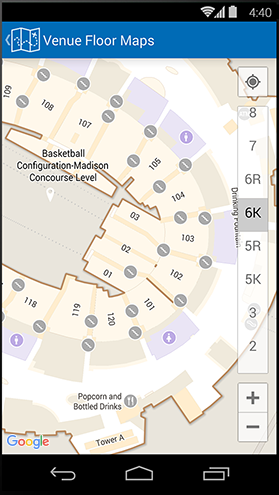
\includegraphics[scale=0.75]{google_indoor_maps_app}
\caption{Screen view of an application using the Google Indoor Maps ~\cite{Google}}
\label{fig:ips_topologies}
\end{figure}
\subsubsection{Competitor Analysis}
An overview of the metrics used to compare competitors:
\begin{enumerate}
\item Ability to read and create digital floor plans from \acrshort{cad} files;
\item Interactive editor to edit digital maps;
\item Wayfinding functionality to declare a \acrlong{poi} and determine routes.
\item Position of the \acrlong{mu} shown on the map;
\item If the company creates the interactive maps itself or if the team of developers need to create it.
\item Customizability of the color scheme and icons;
\item Automation: the degree in which changes and modifications to the architectural structure of the environment translates automatically in a changed digital map.
\item Developer support by providing an \acrshort{api} or \acrshort{sdk};
\item Pricing options;
\item Usability;
\item Additional Features;
\end{enumerate}

\begin{table}[]
\centering
\resizebox{\textwidth}{!}{%
\begin{tabular}{
>{\columncolor[HTML]{ECF4FF}}l llll}
\hline
\cellcolor[HTML]{FFFFFF}                                                     & \cellcolor[HTML]{C0C0C0}\textbf{MapWize}                                                                                                                                                                                         & \cellcolor[HTML]{C0C0C0}\textbf{MazeMap}                                                                                                                             & \cellcolor[HTML]{C0C0C0}\textbf{Google Indoor Maps}                                                               & \cellcolor[HTML]{C0C0C0}\textbf{MapsIndoors}                                                                                                 \\ \hline
\multicolumn{1}{|l|}{\cellcolor[HTML]{ECF4FF}\textit{Convert CAD files}}     & \multicolumn{1}{l|}{Yes}                                                                                                                                                                                                         & \multicolumn{1}{l|}{Yes}                                                                                                                                             & \multicolumn{1}{l|}{No}                                                                                           & \multicolumn{1}{l|}{No}                                                                                                                      \\ \hline
\multicolumn{1}{|l|}{\cellcolor[HTML]{ECF4FF}\textit{Interactive editor}}    & \multicolumn{1}{l|}{Yes}                                                                                                                                                                                                         & \multicolumn{1}{l|}{Yes}                                                                                                                                             & \multicolumn{1}{l|}{Yes}                                                                                          & \multicolumn{1}{l|}{Yes}                                                                                                                     \\ \hline
\multicolumn{1}{|l|}{\cellcolor[HTML]{ECF4FF}\textit{Wayfinding}}            & \multicolumn{1}{l|}{Yes, manual}                                                                                                                                                                                                 & \multicolumn{1}{l|}{Yes, manual}                                                                                                                                     & \multicolumn{1}{l|}{Yes, manual}                                                                                  & \multicolumn{1}{l|}{Yes, manual}                                                                                                             \\ \hline
\multicolumn{1}{|l|}{\cellcolor[HTML]{ECF4FF}\textit{Location tracking}}     & \multicolumn{1}{l|}{Yes}                                                                                                                                                                                                         & \multicolumn{1}{l|}{Yes}                                                                                                                                             & \multicolumn{1}{l|}{Yes}                                                                                          & \multicolumn{1}{l|}{Yes}                                                                                                                     \\ \hline
\multicolumn{1}{|l|}{\cellcolor[HTML]{ECF4FF}\textit{Updates}}               & \multicolumn{1}{l|}{Automated, real-time}                                                                                                                                                                                        & \multicolumn{1}{l|}{Automated, real-time}                                                                                                                            & \multicolumn{1}{l|}{Manual by email}                                                                              & \multicolumn{1}{l|}{Automated, real-time}                                                                                                    \\ \hline
\multicolumn{1}{|l|}{\cellcolor[HTML]{ECF4FF}\textit{Customizability of UI}} & \multicolumn{1}{l|}{Fully customizable}                                                                                                                                                                                          & \multicolumn{1}{l|}{Fully customizable}                                                                                                                              & \multicolumn{1}{l|}{Standard Google Maps UI}                                                                      & \multicolumn{1}{l|}{Fully customizable}                                                                                                      \\ \hline
\multicolumn{1}{|l|}{\cellcolor[HTML]{ECF4FF}\textit{Developer support}}     & \multicolumn{1}{l|}{\begin{tabular}[c]{@{}l@{}}Barebones and UI SDK / API, \\ open source\end{tabular}}                                                                                                                          & \multicolumn{1}{l|}{SDK / API}                                                                                                                                       & \multicolumn{1}{l|}{API}                                                                                          & \multicolumn{1}{l|}{SDK / data API}                                                                                                          \\ \hline
\multicolumn{1}{|l|}{\cellcolor[HTML]{ECF4FF}\textit{Pricing}}               & \multicolumn{1}{l|}{Paid}                                                                                                                                                                                                        & \multicolumn{1}{l|}{Paid}                                                                                                                                            & \multicolumn{1}{l|}{Free}                                                                                         & \multicolumn{1}{l|}{Paid}                                                                                                                    \\ \hline
\multicolumn{1}{|l|}{\cellcolor[HTML]{ECF4FF}\textit{Usability}}             & \multicolumn{1}{l|}{\begin{tabular}[c]{@{}l@{}}Easy to use,\\ integration for iOS, Android\\ and JS\end{tabular}}                                                                                                                & \multicolumn{1}{l|}{\begin{tabular}[c]{@{}l@{}}Easy to use and support for the\\ blind and visually impaired,\\ integration for iOS, Android\\ and JS\end{tabular}}  & \multicolumn{1}{l|}{\begin{tabular}[c]{@{}l@{}}Easy to use,\\ integration for iOS, Android\\ and JS\end{tabular}} & \multicolumn{1}{l|}{\begin{tabular}[c]{@{}l@{}}Easy to integrate in\\ legacy software,\\ integration for iOS, Android\\ and JS\end{tabular}} \\ \hline
\multicolumn{1}{|l|}{\cellcolor[HTML]{ECF4FF}\textit{Additional features}}   & \multicolumn{1}{l|}{\begin{tabular}[c]{@{}l@{}}Private PoI, CMS system,\\ integration of other indoor\\ location technologies,cloud-based \\ or on-premises deployment, integration\\ of IndoorLocation frameworks\end{tabular}} & \multicolumn{1}{l|}{\begin{tabular}[c]{@{}l@{}}IoT platform for asset\\ tracking, system integrations,\\ availability of meeting rooms, private\\ maps\end{tabular}} & \multicolumn{1}{l|}{Standard Google Maps Features}                                                                & \multicolumn{1}{l|}{\begin{tabular}[c]{@{}l@{}}Cloud-based ecosystem\\ with integration for legacy\\ systems\end{tabular}}                   \\ \hline
\end{tabular}%
}
\caption{Comparison of MapWize, MazeMap, Google Indoor Maps and MapsIndoors}
\label{tab:my-table}
\end{table}
\subparagraph{Conclusion}
The differences in features of each competitor are nuanced, each company provides the same basic set of features, where the largest difference will be in price. However, Google Indoor Maps does not provide all the features of MazeMap, MapWize and MapsIndoors, and offers only a bare-bones service, which is not a surprise considering the free usage of the platform. All in all, Google Indoor Maps is a suitable service to use for small-scale applications but cannot be applied to this specific case. The main advantage that MapWize and MazeMap have in comparison to their competitors is the ability to seamlessly integrate Cisco CMX, with MapWize being able to integrate more \acrshort{ips}s such as Meraki, OledComm and Lucibel \cite{IndoorLocation}. The option to host MapWize on-premises can result in a higher performance by eliminating the need to interact with a server outside of the network and allows full control over the MapWize environment. MazeMap would be a great service to use inside 'smart\ building, where multiple sensors and \acrshort{iot}-devices are present. Another great feature of MazeMap is the ability to view meeting rooms and their status (open, booked or free), this is not applicable to the case study in this bachelor's thesis, thus not a feature that can be directly used. If it were to be customizable and applicable to hospital rooms, this would present the hospital with an interesting way to manage and book rooms and/or offices. Both MazeMap and MapWize provide an integration of Cisco \acrshort{cmx} that results in both being well-rounded services to use in this case study.
\subsection{MapWize SDK for Android Applications}
By providing an SDK to aid developers, MapWize hopes to gain an advantage over its competitors. There are currently two different SDKs available:
\begin{enumerate}
\item Bare-bones SDK;
\item UI SDK;
\end{enumerate}
\subsection{MapWize Editor}
To create the interactive map, MapWize provides an editor which enables users to perform the following actions:
\begin{itemize}
\item Create venues;
\item Create multiple floors;
\item Define ~\acrshort{pois};
\item Create one or multiple routes from different locations in the venue to specific ~\acrlong{pois};
\item Export the map;
\item Import \acrshort{cad} files into the map;
\end{itemize}
\section{IndoorLocation Framework in Android}
MapWize itself does not provide a technique to interact with an \acrlong{ips}, they have however partnered with IndoorLocation.io to interact with numerous indoor location applications, such are: Cisco CMX, Cisco Meraki, beco, OledComm, Basic Beacon, Polestar and Lucibel \cite{IndoorLocation}.
\subsection{Integrating IndoorLocation Framework in Android Applications}
To integrate both MapWize (using the \acrshort{ui} \acrshort{sdk}) and IndoorLocation inside an Android \acrshort{app} only a few steps are necessary:
\begin{enumerate}
\item Add MapWize and IndoorLocation dependencies.
\item Create an Application context that instantiates a manager with \acrshort{api} key.
\item Setup the MapActivity, displaying a specific venue.
\item Initiate a socket listener for a Cisco \acrshort{cmx} server to get the position.
\item If needed, add some options to the MapWizeUISettings fragment.
\end{enumerate}
\subsection{Project Setup}
To start working with the MapWize \acrshort{ui} \acrshort{sdk}, an Android project is required. To initiate an Android project, installation of Android Studio is mandatory. In Android Studio a project can be created and then used for further developments.
\subsubsection{Adding the MapWize and IndoorLocation Dependencies}
The dependencies in an Android \acrshort{app} are managed by either gradle or maven, this specfici implementation makes use of gradle 5.4+ and Android Studio 3.4+. To add the dependencies of MapWize and IndoorLocation, simply add the following lines to the build.gradle file under the dependencies section of the project:
\begin{verbatim}
 // MAPWIZE
implementation('io.mapwize.indoormaps:MapwizeForMapbox:2.0+') {
	exclude group: 'com.github.IndoorLocation', module: 'indoor-location-android'
	transitive = true
}
implementation 'com.github.IndoorLocation:indoor-location-android:1.0.5'
implementation('io.socket:socket.io-client:1.0.0') {
	exclude group: 'org.json', module: 'json'
}
mplementation 'com.github.Mapwize:mapwize-ui-android:1.2.0'
\end{verbatim}
\subsubsection{Creating an Application Context}
The code below creates a child class of the Application base class and overrides the onCreate() method.
\begin{verbatim}
public class MapApplication extends Application {

    @Override
    public void onCreate() {
        super.onCreate();
        AccountManager.start(this, "1f04d780dc30b774c0c10f53e3c7d4ea");// PASTE YOU MAPWIZE API KEY HERE !!! This is a demo key, giving you access to the demo building. It is not allowed to use it for production. The key might change at any time without notice. Get your key by signin up at mapwize.io
    }
}
\end{verbatim}
To automatically run the application using the custom MapWizeApplication, the following code needs to be present in the AndroidManifest.xml file of the Android \acrshort{app}:
\begin{verbatim}
<application
        android:allowBackup="true"
        android:icon="@mipmap/ic_launcher"
        android:label="@string/app_name"
        android:roundIcon="@mipmap/ic_launcher_round"
        android:supportsRtl="true"
        android:theme="@style/AppTheme"
        android:name=".MapApplication">
        <activity android:name=".MapActivity">
            <intent-filter>
                <action android:name="android.intent.action.MAIN" />

                <category android:name="android.intent.category.LAUNCHER" />
            </intent-filter>
        </activity>
    </application>
\end{verbatim}
\subsubsection{MapActivity}
Appendix 1 shows the complete code of the MapActivity that contains the following fields:
\begin{itemize}
\item A fragment for displaying the map: mapwizeFragment;
\item The SocketIndoorLocationProvider to integrate the IndoorLocation framework in the activity: socketIndoorLocationProvider;
\item The plugin provided by the MapWize \acrshort{sdk}: mapwizePlugin;
\item To display the map, the field that holds a MapboxMap is created: mapboxMap;
\end{itemize}
The basic options used in the example \acrshort{app} are: restricting view of the map to a specific venue, showing the menu button and the follow user button. Upon adding the mapwizeFragment to a specific container, the event onFragmentready is fired, where the mapboxMap and mapwizePlugin are set for this particular activity. Afterwards, the socketIndoorLocationProvider is instantiated with an IP address, that of the emitter of the position of the \acrlong{mu}. This provider is then set as a property of the mapwizePlugin and afterwards the provider is started. To follow the user when moving, the FollowUserMode is set and the mapwizePlugin gets the user position by calling that method. When implementing the MapWize \acrshort{sdk}, some methods are required to be implemented:
\begin{itemize}
\item shouldDisplayInformationbutton: whether or not the information button needs to be displayed.
\item shouldDisplayFloorController: if a user should be able to control the view of different floors;
\item onFollowUserButtonClickWithoutLocation: if anything needs to happen when a user clicks the the follow button without having granted access to his or her location, this is handy for displaying errors to the \acrshort{mu}.
\item onInformationButtonClick: this event can be used to display information on a specific venue when the user clicks on the corresponding button.
\item onrequestPermissionsResult:
\end{itemize}
\section{Conclusion}
The integration of MapWize and the IndoorLocation went without any actual errors coming up. It is easy to combine both MapWize and IndoorLocation as the \acrshort{sdk} already contains the necessary boilerplate code to generate a \acrlong{ui}. The implementation of the barebones \acrshort{sdk} would require a lot of additional steps to connect the \acrshort{ui} with the code. It would also be difficult to correctly handle the specific events that are able to be fired during the lifecycle of the application. Problems such as optimizing performance, rendering the \acrshort{ui}, handling the lifecycle of the \acrshort{app} are already solved in the \acrshort{ui} \acrshort{sdk}. This implementation concluded in a straightforward way of integration Cisco \acrshort{cmx} indoor location in an Android \acrshort{app}.